\chapter{利用掩食搜索双星中的星周盘} \label{chapter:form_evo}

\section{研究背景} \label{sec:diskbackground}

\subsection{星周盘简介} \label{sec:diskintro}

盘在天体物理中十分常见:从星系尺度的气体盘\cite{Binney1987,Gilmore1989}到致密星周围的吸积盘
\cite{Pringle1981},再小至行星形成的原行星盘(\S \ref{sec:pltfrmatntheory})以及形成卫星摇篮 --- 环
行星盘\cite{Smith1981,Latter2017,Mosqueira2003}。早在 17 世纪初盘,笛卡尔为了解释太阳系的行星
构型就引入了盘的概念,尽管那时候人类并未真正了解原恒星盘的模样\cite{Kawabe1993}。如今已迈入
中年的太阳系依然尚有黄道尘埃盘\cite{Dermott1994}、主小行星带以及库依柏带星子盘,这些也都是太
阳系纷乱的历史留下的残骸\cite{Dohnanyi1969}。


\begin{figure}[b]
\centering
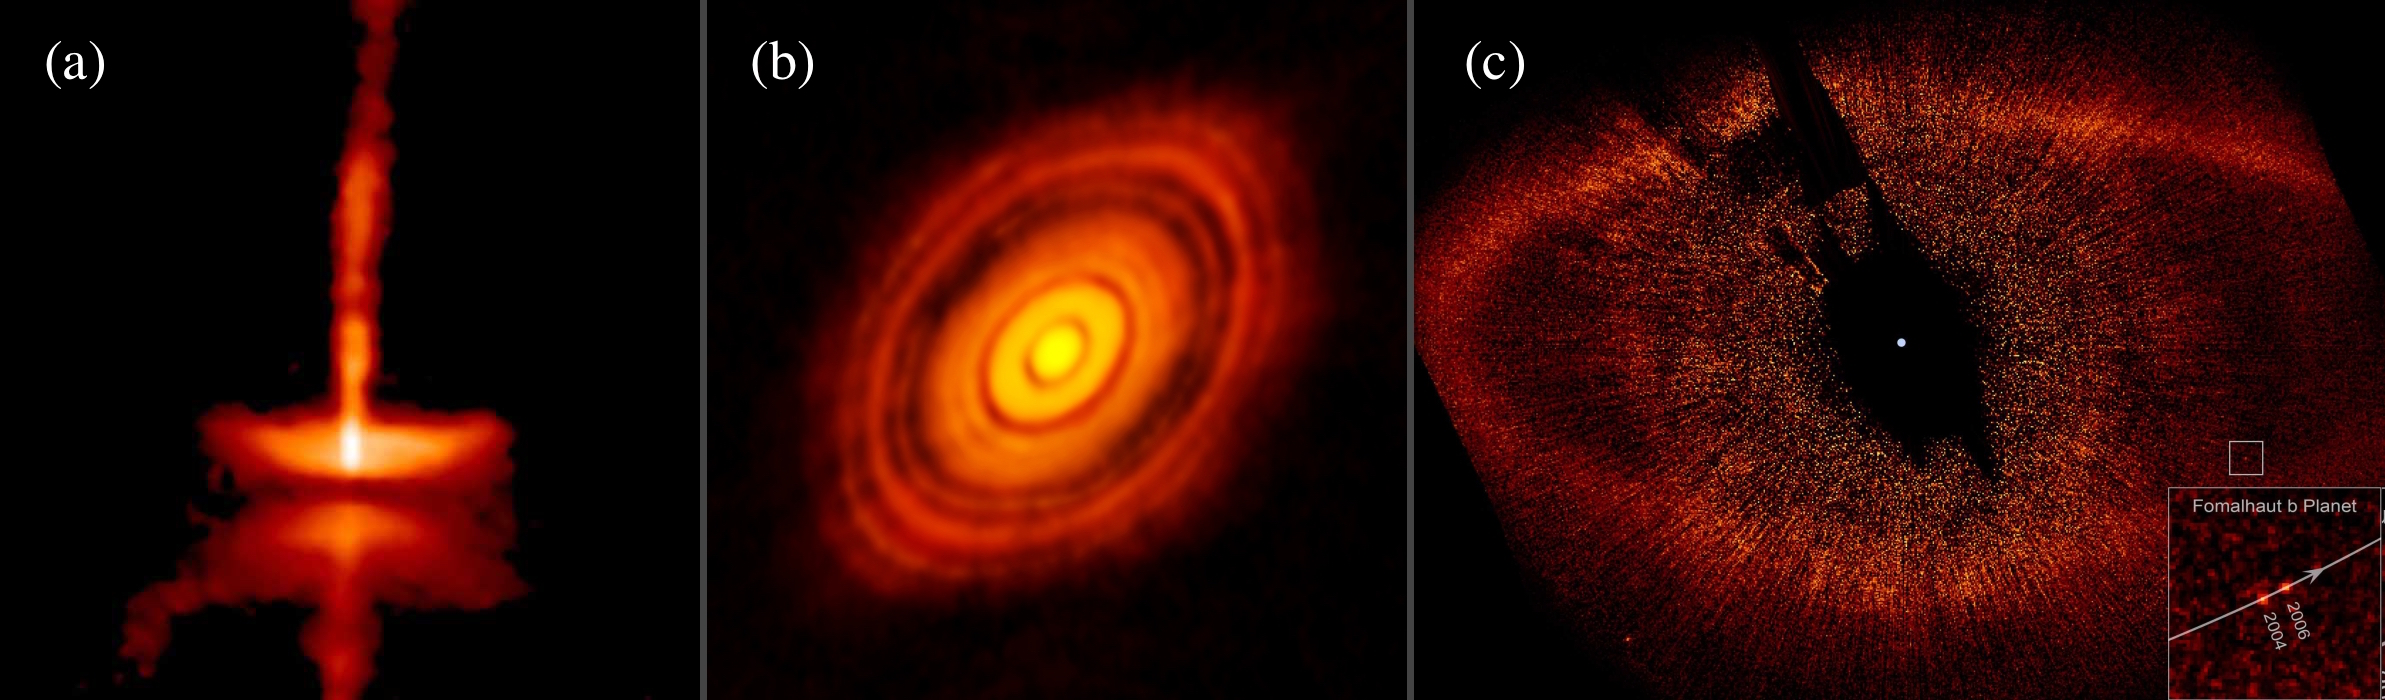
\includegraphics[width=1.0\textwidth]{figures/chapter3/f2_obsdisc.jpg}
\caption{原行星盘从早期到晚期不同的形态,其中 \textbf{(a)} HH 30 侧向视角的临变增厚盘,双极喷流清晰可见(版权:NASA, Alan Watson) \textbf{(b)} HL Tau (版权:ALMA - ESO/NAOJ/NRAO) \textbf{(c)} Formalhaut 残骸盘(版权:NASA,ESA 和 P. Kalas 等)。}
\label{fig:obsdisc}
\end{figure}


正如前文(参考\S \ref{sec:pltfrmatntheory})提到,行星孕育在星周盘内。此过程(如图 \ref{fig:pfdics} 与 \ref{fig:obsdisc} 所示)包括早期分子云坍缩、恒星吸积盘内固体沉降、气体消散行星形成和最终演化为残骸盘(Debris disk,又称碎屑盘)几个阶段。一般而言,描述气体的过程为内盘区域等离子磁层作用与外层气体辐射转移两个过程\cite{Dullemond2010,WilliamsCieza2011},而脱离气体耦合作用后的固体盘一般则为 N 体引力作用(\S \ref{sec:clspftheory})。


\begin{sidewaysfigure}
\centering
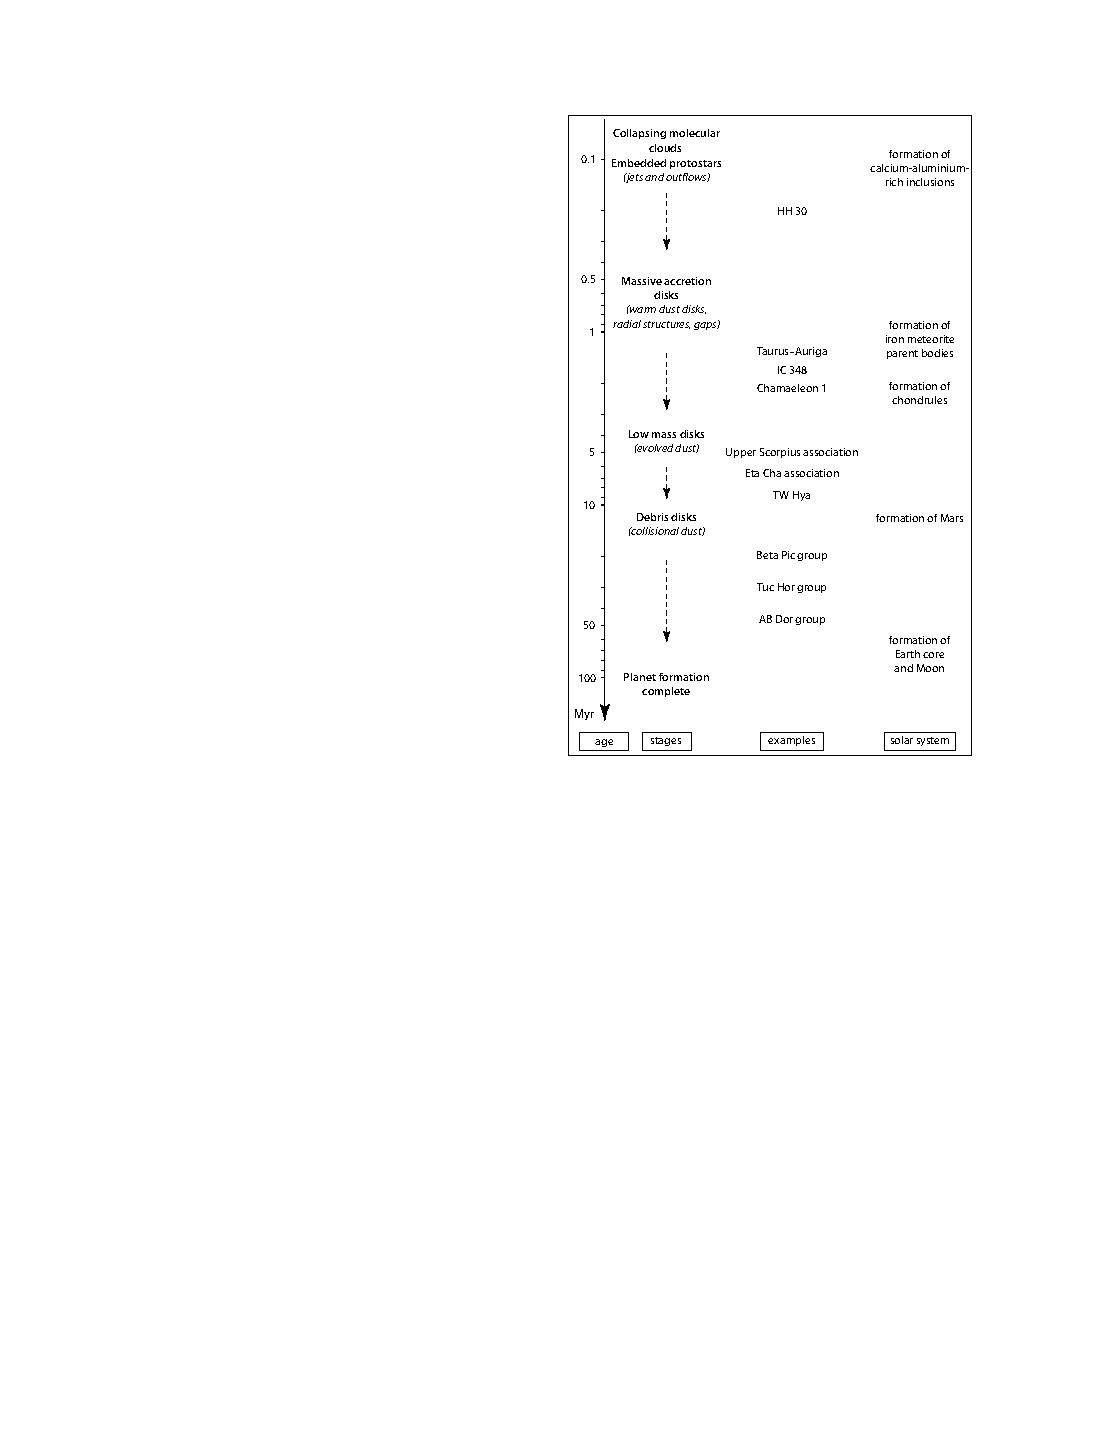
\includegraphics[scale=3.0, angle=-90]{figures/chapter3/f1_pfdisc.pdf}
\caption[行星形成的不同时期快照,从左至右分别为时间、形成阶段、系外行星系统实例与太阳系历史,版权所有人 Perryman。]{行星形成的不同时期快照,从左至右分别为时间、形成阶段、系外行星系统实例与太阳系历史。图片采取自书籍\citen{Perryman2014exohb},更详细的图请查看书籍\ref{ApaiLauretta2010}。}
\label{fig:pfdics}
\end{sidewaysfigure}



星周盘(Circumstellar disk)观测到的辐射在理论上一般会用多黑体辐射谱来拟合。普朗克黑体谱(Black body)有如下形式:

\begin{equation} \label{eq:blackbody}
\tif{B}_\nu (\tif{T}) = \frac{2h\nu^3}{c^2} \, \frac{1}{e^{h\nu / k\tif{T}}-1}
\end{equation} %myequation{黑体辐射}


同样,径向对称且几何薄的星周盘总辐射可看作每个环状细盘黑体辐射的积分叠加,形式如下:

\begin{equation} \label{eq:diskrad}
\tif{F}_\nu = \frac{\cos \theta}{\tif{D}^2} \, \int \tif{B}_\nu (\tif{T}_\tif{d}) \, ( 1-e^{-\tau} ) 2\pi r \tif{d} r \ ,  
\end{equation} %myequation{盘总辐射量}
其中 $\theta$ 为观测者的视角,D 为观测者和源之间的距离。光深 $\tau$ 与盘内尘埃的不透明度(Opacity)以及盘的面密度分布有关。星周盘的尘埃辐射主要集中在红外或更长的波段,所以观测中一般将上述流量描述为红外光度比例 $\tif{L}_\tif{IR}/\tif{L}_\tif{s}$,即使用星周盘谱能量分布(SED)函数来简化(参考图 \ref{fig:transdiscsed} 和图 \ref{fig:debrisdiscsed})。


\begin{figure}[t]
\centering
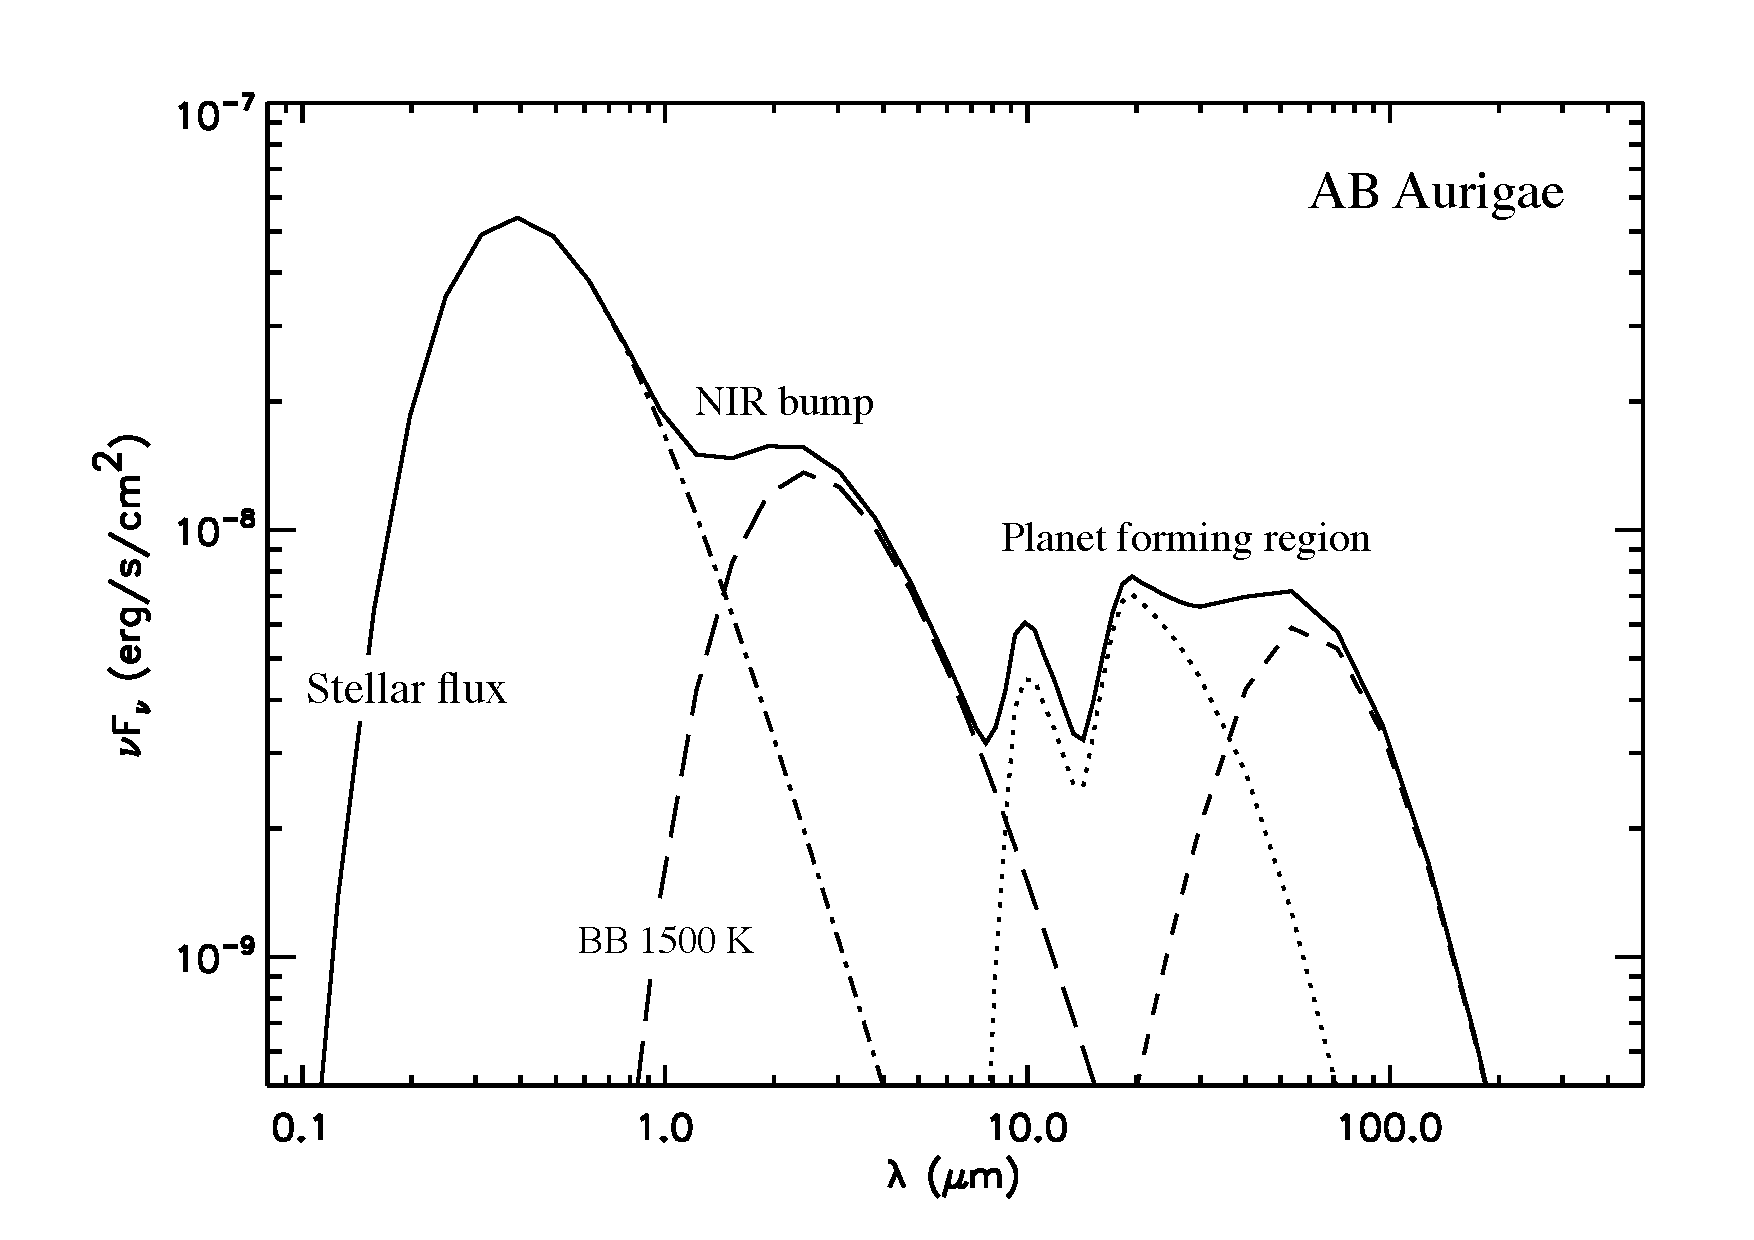
\includegraphics[width=1.0\textwidth]{figures/chapter3/f3_youngdisc.pdf}
\caption[AB Aurigae 系统理论谱能量分布图。从左至右分别表示恒星、有效温度为 1500 K 的星周内侧盘与外侧行星形成区域的黑体辐射组分。该图利用 Dullemond 开发的 CGPlus 程序制作。]{AB Aurigae 系统理论谱能量分布图。从左至右分别表示恒星、有效温度为 1500 K 的星周内侧盘与外侧行星形成区域的黑体辐射组分。此图利用 Dullemond 开发的 CGPlus 程序\footnotemark[1]制作。}
\label{fig:transdiscsed}
\setcounter{footnote}{1}
\addtocounter{footnote}{+0}\footnotetext{链接 \url{http://www.mpia.de/homes/dullemon/radtrans/fitcgplus/}。}
\end{figure}


\begin{figure}[t]
\centering
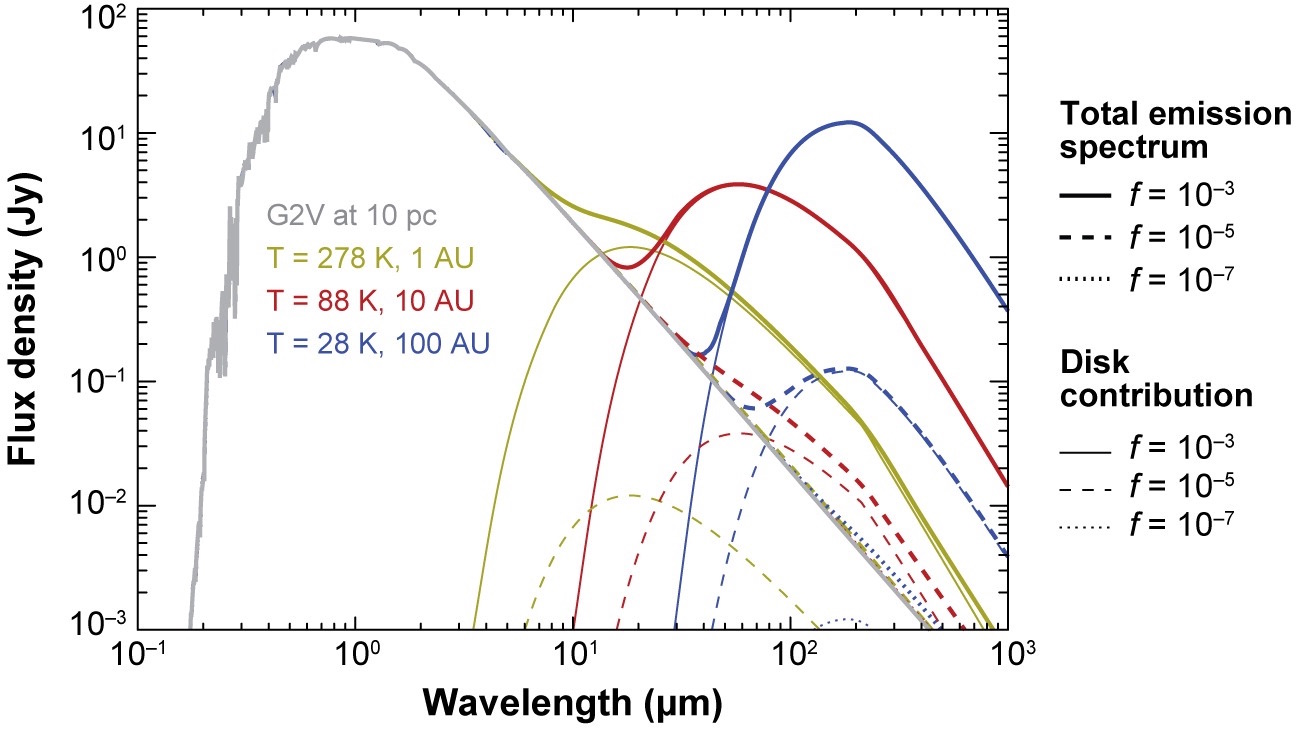
\includegraphics[width=1.0\textwidth]{figures/chapter3/f4_debrisdisc.jpg}
\caption[类太阳(G2V)恒星于 10 pc 以外的理论辐射谱能量函数,长波范围的鼓包为星周残骸盘的黑体辐射。图片版权归 Wyatt 所有。]{类太阳(G2V)恒星于 10 pc 以外的理论辐射谱能量函数,长波范围的鼓包为星周残骸盘的黑体辐射。图片取自文献\citen{Wyatt2008}。}
\label{fig:debrisdiscsed}
\end{figure}


\subsection{双星中星周盘研究背景} \label{sec:diskintro}

Binary stellar systems



\section{利用 EB 掩食光变曲线搜索星周盘} \label{sec:diskintro}


